\section{Υλοποιημένα παραδείγματα\cite{dummy}}
\subparagraph{}
Οι ενότητες που ακολουθούν αφορούν την επίλυση προβλημάτων με διαφορετικές μεθόδους. Τα προβλήματα συγκεντρώθηκαν και επιλύθηκαν με στόχο την σύγκριση των αποτελεσμάτων και την εξαγωγή συμπερασμάτων σε επίπεδο χρονικής επίδοσης. Παράλληλα θα σχολιαστούν επιμέρους οι διάφορες παραλλαγές επίλυσης του κάθε προβλήματος. Ο πηγαίος βρίσκεται συγκεντρωμένος στον παρακάτω σύνδεσμο: $$\href{https://github.com/gkonto/openmp/}{\en{https://github.com/gkonto/openmp/}}$$
Κάθε πρόβλημα περιέχει υποφακέλους και κάθε υποφάκελος αποτελεί μια παραλλαγή του προβλήματος.
\begin{center}

\begin{figure}[h]
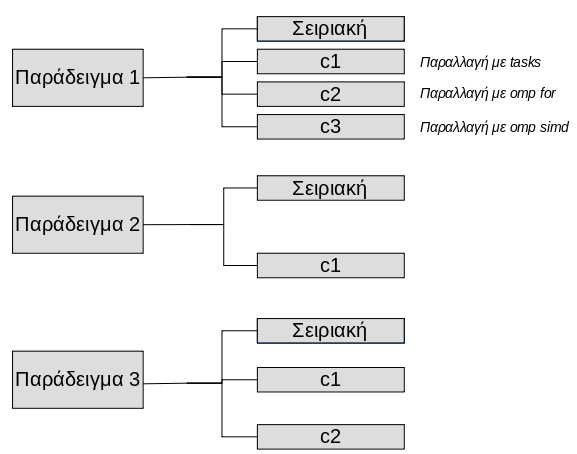
\includegraphics[width=\textwidth]{diarthrosi_example}
\captionsetup{justification=centering, singlelinecheck=false}
\caption{Διάρθρωση παραδειγμάτων στο \href{https://github.com/gkonto/openmp/}{\emph{\en{github.com}}}}
\label{fig:diarthrosi_example}
\end{figure}
\end{center}

\clearpage
\subsection{Αναφορά αρχιτεκτονικής μηχανήματος}
\subparagraph{}
\ \\
Τα προβλήματα που ακολουθούν εκτελέστηκαν σε μηχάνημα λειτουργικό \emph{\en{linux}} και μεταγλωττιστή \emph{\en{gcc}}. Οι προδιαγραφές υλικού του μηχανήματος που εκτελέστηκαν τα προβλήματα, αναφέρονται στο παρακάτω παράδειγμα:

\selectlanguage{greek}
\begin{center}
\begin{table}[htbp]
\centering
\captionsetup{justification=raggedright,
singlelinecheck=false
}
\caption{Χαρακτηριστικά Μηχανήματος Εκτέλεσης}
\def\arraystretch{1.5}
\begin{tabular}{| p{0.25\textwidth} | p{0.25\textwidth}|}
\hline
 \en{\textbf{Architecture}}  \cellcolor[HTML]{D0D0D0} & \en{x86\_64}  \\
\hline
 \en{\textbf{CPU op-mode(s)}} \cellcolor[HTML]{D0D0D0} & \en{32-bit, 64-bit} \\
\hline
 \en{\textbf{CPU(s)}} \cellcolor[HTML]{D0D0D0}  & 16\\
\hline
 \en{\textbf{Thread(s) per core}} \cellcolor[HTML]{D0D0D0} & 1 \\
\hline
 \en{\textbf{Core(s) per socket}} \cellcolor[HTML]{D0D0D0} & 8\\
\hline
 \en{\textbf{Socket(s)}} \cellcolor[HTML]{D0D0D0} & 2 \\
\hline
 \en{\textbf{NUMA node(s)}} \cellcolor[HTML]{D0D0D0} & 4\\
\hline
 \en{\textbf{Model name}} \cellcolor[HTML]{D0D0D0}  &  \en{AMD Opteron(tm) Processor 6128 HE}\\
\hline
\en{\textbf{L1d cache}} \cellcolor[HTML]{D0D0D0} &  \en{64K} \\
\hline
\en{\textbf{L2 cache}} \cellcolor[HTML]{D0D0D0} & \en{512K}  \\
\hline
\en{\textbf{L3 cache}} \cellcolor[HTML]{D0D0D0} & \en{5118K}  \\
\hline
 \en{\textbf{Memory}} \cellcolor[HTML]{D0D0D0} & 16036\\
\hline
\end{tabular}
\end{table}
\end{center}

\clearpage